\documentclass[11pt, a4paper]{article}
\usepackage[top=2cm, bottom=2cm, left=2cm, right=2cm]{geometry}
\usepackage[english]{babel}
\usepackage[T1]{fontenc}
\usepackage[utf8x]{inputenc}
\usepackage{mathtools}
\usepackage{amsfonts}
\usepackage{amssymb}
\usepackage{array}
\usepackage{booktabs}
\usepackage{float}
\usepackage{algorithm}
\usepackage{algpseudocode}
\usepackage{hyperref}
\usepackage{tikz}
\usepackage{xfrac}
\usepackage{xcolor}
\usepackage{longtable}
\usepackage[font=footnotesize, labelfont=bf, margin=30pt]{caption}
\usepackage[font=scriptsize, labelfont=bf, margin=30pt]{subcaption}

\usetikzlibrary{trees, arrows}

\author{Francesco Landolfi \and Giorgio Vinciguerra}
\title{Exercises of Information Retrieval}

\newcommand{\exercise}{\subsection{Exercise} \paragraph{Question}}
\newcommand{\solution}{\paragraph{Solution}}
\newcommand{\hl}[1]{\colorbox{yellow}{#1}}

\begin{document}
\maketitle
% \clearpage
% --------------- DO NOT EDIT --------------- %
% This file has been automatically generated. %

\section{Introduction}
\exercise

Given the inverted lists of two terms $t_1$ and $t_2$, write the pseudo-code of the
algorithm that implements $t_1$ AND (NOT $t_2$). Discuss and compute its time
complexity as a function of the lengths of the two posting lists.  \emph{(Hint:
do not create explicitly (NOT $t_2$))}

\solution

Given $m = |t_1|$ and $n = |t_2|$, the following algorithm takes
$\mathcal{O}(m+n)$ time in the worst case, while $\mathcal{O}(m)$ in the best
case (i.e., when $\max\{t_1\} < \min\{t_2\}$). This algorithm performs a scan of
both lists, so the I/O complexity is $\mathcal{O}(\frac{m}{B}+\frac{n}{B})$.
Both complexities may be improved using skip pointers.

\begin{algorithm}[H]
\caption{}\label{alg:andnot}
\begin{algorithmic}[1]
\Function{AndNot}{$p_1$, $p_2$}
\State $res \gets \langle\rangle$
\While{$p_1 \neq nil$}
\If{$p_2 = nil$}
\State $res.\text{\scshape appendAll}(p_1)$
\ElsIf{$p_1.id < p_2.id$}
\State $res.\text{\scshape append}(p_1.id)$
\State $p_1 \gets p_1.next$
\ElsIf{$p_1.id = p_2.id$}
\State $p_1 \gets p_1.next$
\State $p_2 \gets p_2.next$
\Else
\State $p_2 \gets p_2.next$
\EndIf
\EndWhile
\State \Return $res$
\EndFunction
\end{algorithmic}
\end{algorithm}

\section{Crawling}
\exercise

Given a dictionary of $2^{16}$ strings,
%
\begin{itemize}

  \item compute the error rate of a Bloom Filter which uses an array of $2^{20}$
  bits and an optimal number of hash functions \emph{(assume that logs are in
  base 2)};

  \item say when the use of the Bloom Filter is advantageous in space with
  respect to the use of a standard hash table, given that the strings have
  length $L$ bits each and pointers cost 32 bits each.

\end{itemize}

\solution

The optimal number of hash functions is given by
%
\begin{align*}
  k = \frac{m}{n}\ln 2 = 2^4 \ln 2
\end{align*}
%
while the error rate is given by
%
\begin{align*}
  \varepsilon = \left( 1 - e^{-\frac{kn}{m}}\right)^k \approx 0.618^{16}.
\end{align*}

Regarding the second point, if we use an hash table then, only for the
initialization (\emph{without inserting any string in the dictionary}), for each
of its slot we have to allocate 2 pointers (one for the string, one for the
bucket), so $64 \cdot 2^d$ bits, where $d$ is the dimension of the dictionary.
For the Bloom Filter, instead, we have to allocate just $2^d$ bits, so the hash
table is alway disadvantageous.

\exercise

Compute the probability of error for a Bloom Filter that uses a bit-array of $m$
bits, $k$ hash functions and indexes a dictionary of $n$ strings.

\solution

The probability that a bit in the array $\mathbf{b}$ is 1 after $n$ insertions
is
%
\begin{align*}
  \mathbb{P}[\mathbf{b}_i^{(n)} = 1] &= 1 - \mathbb{P}[\mathbf{b}_i^{(n)} = 0]\\
  &= 1 - \left( 1 - \frac{1}{m} \right)^{kn} \\
  &\approx 1 - e^{-\frac{kn}{m}}
\end{align*}
%
Then, the probability of a false positive for a given vector $\mathbf{v}$ is:
%
\begin{align*}
  \mathbb{P}[\mathbf{b}_{h_1(\mathbf{v})}^{(n)} = 1 \wedge \dots \wedge
  \mathbf{b}_{h_k(\mathbf{v})}^{(n)} = 1] &= \left(1 - \left( 1 - \frac{1}{m}
  \right)^{kn} \right)^k \\ &\approx \left(1 - e^{-\frac{kn}{m}} \right)^k
\end{align*}

\exercise

Assume that you have 7 items (6, 1, 3, 7, 2, 4, 9) and three servers whose IDs
are (1, 2, 3), and you want to distribute those items among the three servers
via consistent hashing. How would you do? What if a new server with ID 11 goes
up? \emph{(Hint: Instead of working on ring $[0,1]$, work on the integers in
$\{0,1, ... ,10\}$ using a universal hash function $h_a(x)= a*x \bmod m)$}

\solution

Given $a = 3$ we obtain that $h_3(1) = 3$, $h_3(2) = 6$, $h_3(3) = 9$. The items will be distributed as in the following table:
%
\begin{table}[h]
  \centering
  \begin{tabular}{l|c|c|c|c|c|c|c}
    item & 6 & 1 & 3 & 7 & 2 & 4 & 9 \\
    $h_3(\text{item})$ & 7 & 3 & 9 & 10 & 6 & 1 & 5 \\ \hline
    server ID & 3 & 1 & 3 & 1 & 2 & 1 & 2 \\
  \end{tabular}
\end{table}

If a new server with ID = 11 (and $h_3(11) = 0$) goes up, the item 7 will be
reassigned to that server.

\exercise

Consider the Consistent Hashing technique,
%
\begin{enumerate}

  \item simulate its execution over the $id_{url} = \{ 1, 2, 4, 6, 7, 8, 11,
  13 \}$ and the $id_{crawler} = \{ 2, 4, 7 \}$, by defining the hash function
  $h_3(x) = 3x \bmod 11$;

  \item Show what happens if the $id_{crawler}$ 2 faults.

\end{enumerate}

\solution

\begin{enumerate}

  \item First, w compute the hashes of the $id_{crawler}$ and we obtain that
  $h_3(2) = 6$, $h_3(4) = 1$, $h_3(7) = 10$. The items will be distributed as in
  the following table:
  %
  \begin{table}[h]
    \centering
    \begin{tabular}{l|c|c|c|c|c|c|c|c}
      $id_{url}$      & 1 & 2 & 4 & 6 & 7 & 8 & 11 & 13 \\
      $h_3(id_{url})$ & 3 & 6 & 1 & 7 & 10 & 2 & 0 & 6 \\ \hline
      $id_{crawler}$  & 2 & 2 & 4 & 7 & 7 & 2 & 4 & 2 \\
    \end{tabular}
  \end{table}

  \item If the crawler with $id_{crawler}$ 2 faults, the items with $id_{url}$
  1, 2, 8, and 13 will be reassigned to $id_{crawler}$ 7.

\end{enumerate}

\section{Locality-Sensitive Hashing}
\exercise

Given a set of binary vectors,
%
\begin{enumerate}

  \item describe how it is computed an LSH-fingerprint of a binary vector
  \textbf{v} to fast to approximate the Hamming distance between vector-pairs
  with high probability \emph{(Hint: state clearly the parameters involved in
  the setting)};

  \item state and prove how the Hamming distance between two vectors \textbf{v}
  and \textbf{w} is related to the probability of declaring a “match” between
  LSH-fingerprints of \textbf{v} and \textbf{w}, according to the various
  parameters involved;

  \item apply your description on the set of vectors $V = \{00000, 00100,
  01010\}$, and use it to estimate Hamming(00000, 01010) and Hamming(00000,
  00100).

\end{enumerate}

\solution

\begin{enumerate}

  \item We compute a sketch of all the vectors of the set via LSH: for each
  vector we take $L$ $k$-projections $h_1$, $h_2$, \dots, $h_L$ and generate
  %
  \begin{align*}
    g(\textbf{u}) = \langle h_1(\textbf{u}), h_2(\textbf{u}), \dots,
    h_L(\textbf{u}) \rangle
  \end{align*}
  %
  We know that, for every $i = 1, \dots, L$ and for every $\mathbf{v, w} \in V$
  it holds that
  %
  \begin{align}\label{eq:lsh-p1}
    \mathbb{P}[h_i(\textbf{v}) = h_i(\textbf{w})] =
    \left( 1 - \frac{d_H(\textbf{v}, \textbf{w})}{n} \right)^k
  \end{align}
  %
  where $n = |\textbf{v}| = |\textbf{w}|$ and $d_H(\textbf{v}, \textbf{w})$ is
  the Hamming distance between $\textbf{v}$ and $\textbf{w}$. We can make an
  empirical estimation of the previous probability with
  %
  \begin{align}\label{eq:lsh-p2}
    \mathbb{P}[h_i(\textbf{v}) = h_i(\textbf{w})] \approx
    1 - \frac{d_H(g(\textbf{v}), g(\textbf{w}))}{L}.
  \end{align}
  %
  We can then combine \autoref{eq:lsh-p1} and \ref{eq:lsh-p2} and get the
  Hamming distance:
  %
  \begin{align*}
    d_H(\textbf{v}, \textbf{w}) &= n \cdot \left( 1 -
    \sqrt[k]{\mathbb{P}[h_i(\textbf{v}) = h_i(\textbf{w})]}\right) \\
    &\approx n \cdot \left( 1 - \sqrt[k]{1 - \frac{d_H(g(\textbf{v}),
    g(\textbf{w}))}{L}}\right)
  \end{align*}

  \item Two fingerprints match ($g(\textbf{v}) \simeq g(\textbf{w})$) if they
  share at least a component in the same position, and the relation between the
  probability of a match and the Hamming distance is
  %
  \begin{align*}
    \mathbb{P}[g(\textbf{v}) \simeq g(\textbf{w})] = 1 - \left( 1 - \left( 1 -
    \frac{d_H(\textbf{v}, \textbf{w})}{n} \right)^k \right)^L
  \end{align*}

  \paragraph{Proof} The probability that, given two vectors $\textbf{v}$ and
  $\textbf{w}$, they share the same bit at the same index $j$ is
  %
  \begin{align*}
    \mathbb{P}[\textbf{v}_j = \textbf{w}_j] = 1 - \frac{d_H(\textbf{v},
    \textbf{w})}{n}.
  \end{align*}
  %
  The probability that the same two vectors share $k$ positions is
  %
  \begin{align*}
    \mathbb{P}[\textbf{v}_{i_1} = \textbf{w}_{i_1} \wedge \dots \wedge
    \textbf{v}_{i_k} = \textbf{w}_{i_k}]
    &= \mathbb{P}[h_i(\textbf{v}) = h_i(\textbf{w})] \\
    &= \left( \mathbb{P}[\textbf{v}_j = \textbf{w}_j] \right)^k \\
    &= \left( 1 - \frac{d_H(\textbf{v}, \textbf{w})}{n} \right)^k.
  \end{align*}
  %
  The probability that at least 1 bit is different is
  %
  \begin{align*}
    \mathbb{P}[\textbf{v}_{i_1} \neq \textbf{w}_{i_1} \vee \dots \vee
    \textbf{v}_{i_k} \neq \textbf{w}_{i_k}]
    &= \mathbb{P}[h_i(\textbf{v}) \neq h_i(\textbf{w})] \\
    &= 1 - \mathbb{P}[h_i(\textbf{v}) = h_i(\textbf{w})] \\
    &= 1 - \left( 1 - \frac{d_H(\textbf{v}, \textbf{w})}{n} \right)^k.
  \end{align*}
  %
  The probability that this will happen for all $L$ projections is
  %
  \begin{align*}
    &\mathbb{P}[h_1(\textbf{v}) \neq h_1(\textbf{w}) \wedge \dots \wedge
    h_L(\textbf{v}) \neq h_L(\textbf{w})] \\ = &\left(
    \mathbb{P}[h_i(\textbf{v}) \neq h_i(\textbf{w})] \right)^L \\ = &\left( 1 -
    \left( 1 - \frac{d_H(\textbf{v}, \textbf{w})}{n} \right)^k \right)^L.
  \end{align*}
  %
  Finally, the probability that at least a projection is shared is
  %
  \begin{align*}
    \mathbb{P}[g(\textbf{v}) \simeq g(\textbf{w})] &=
    \mathbb{P}[h_1(\textbf{v}) = h_1(\textbf{w}) \vee \dots \vee
    h_L(\textbf{v}) = h_L(\textbf{w})] \\ &= 1 -\mathbb{P}[h_1(\textbf{v}) \neq
    h_1(\textbf{w}) \wedge \dots \wedge h_L(\textbf{v}) \neq h_L(\textbf{w})] \\
    &= 1 - \left(\mathbb{P}[h_i(\textbf{v}) \neq h_i(\textbf{w})] \right)^L \\
    &= 1 - \left( 1 -\left( 1 - \frac{d_H(\textbf{v}, \textbf{w})}{n} \right)^k
    \right)^L.
  \end{align*}

  \item Given $V = \{00000, 00100, 01010\}$, we use LSH with parameters $L = 2$
  and $k = 2$. We choose the projections $I_1 = \{ 0, 2 \}$, $I_2 = \{ 3, 4
  \}$ and $I_3 = \{1, 3 \}$ and we obtain the following sketches:
  %
  \begin{table}[H]
    \centering
    \begin{tabular}{c|c|c|c|}
      & $I_1$ & $I_2$ & $I_3$ \\ \hline
      $\mathbf{v_1}$ & 00 & 00 & 00\\ \hline
      $\mathbf{v_2}$ & 01 & 00 & 00\\ \hline
      $\mathbf{v_3}$ & 00 & 10 & 11\\ \hline
    \end{tabular}
  \end{table}
  %
  Then, we compute the Hamming distances between the sketches:
  %
  \begin{table}[H]
    \centering
    \begin{tabular}{c|c|c|c|}
      & $g(\mathbf{v_1})$ & $g(\mathbf{v_2})$ & $g(\mathbf{v_3})$ \\ \hline
      $g(\mathbf{v_1})$ & 0 & 1 & 2 \\ \hline
      $g(\mathbf{v_2})$ & 1 & 0 & 3 \\ \hline
      $g(\mathbf{v_3})$ & 2 & 3 & 0 \\ \hline
    \end{tabular}
  \end{table}
  %
  We can now estimate the Hamming distances between the original vectors:
  %
  \begin{align*}
    d_H(\mathbf{v}_1, \mathbf{v}_2) &\approx
    n \cdot \left( 1 - \sqrt[k]{1 - \frac{d_H(g(\mathbf{v}_1),
    g(\mathbf{v}_2)}{L}} \right) \\
    &= 5 \cdot \left( 1 - \sqrt{1 - \frac{1}{3}} \right) \approx 0.918
    \approx 1 \\
    d_H(\mathbf{v}_1, \mathbf{v}_3) &\approx
    n \cdot \left( 1 - \sqrt[k]{1 - \frac{d_H(g(\mathbf{v}_1),
    g(\mathbf{v}_3)}{L}} \right) \\
    &= 5 \cdot \left( 1 - \sqrt{1 - \frac{2}{3}} \right) \approx 2.113
    \approx 2 \\
    d_H(\mathbf{v}_2, \mathbf{v}_3) &\approx
    n \cdot \left( 1 - \sqrt[k]{1 - \frac{d_H(g(\mathbf{v}_2),
    g(\mathbf{v}_3)}{L}} \right) \\
    &= 5 \cdot \left( 1 - \sqrt{1 - \frac{3}{3}} \right) = 5\ (\neq 3) \\
  \end{align*}

\end{enumerate}

\exercise

Given the binary vectors A = 10111, B = 10010, C = 00010, D = 00000 and E =
01100, apply LSH to find the similar vectors according to Hamming distance,
given $k = 2$ and $L = 2$. \emph{(Hint: use projections $I_1 = \{0, 3\}$, $I_2 =
\{3, 4\}$)}

\solution

First, we construct the sketch of each vector:
%
\begin{figure}[H]
  \hfill
  \begin{minipage}{0.45\columnwidth}
  \centering
  \begin{tabular}{c|c|c}
    {\bf v} & $I_1(\text{\bf v})$ & $I_2(\text{\bf v})$ \\ \hline
    A & 11 & 11 \\
    B & 11 & 10 \\
    C & 01 & 10 \\
    D & 00 & 00 \\
    E & 00 & 00 \\
  \end{tabular}
  \end{minipage}
  \begin{minipage}{0.45\columnwidth}
  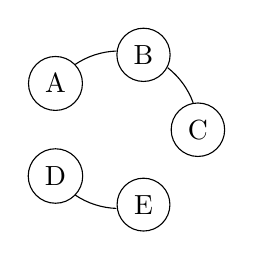
\begin{tikzpicture}
    \centering
    \def \radius {1cm}
    \def \margin {20}

    \node[draw, circle] at (0:\radius) {C};
    \draw[-, >=latex] ({0+\margin}:\radius)
      arc ({0+\margin}:{72-\margin}:\radius);
    \node[draw, circle] at (72:\radius) {B};
    \draw[-, >=latex] ({72+\margin}:\radius)
      arc ({72+\margin}:{144-\margin}:\radius);
    \node[draw, circle] at (144:\radius) {A};
    \node[draw, circle] at (216:\radius) {D};
    \draw[-, >=latex] ({216+\margin}:\radius)
      arc ({216+\margin}:{288-\margin}:\radius);
    \node[draw, circle] at (288:\radius) {E};

  \end{tikzpicture}
  \end{minipage}
  \hfill
\end{figure}
%
By the previous table, we can construct the similarity graph and conclude that:
%
\begin{itemize}
  \item A, B, C are similar;
  \item D, E are similar.
\end{itemize}

Alternatively, to speed up query time, we can construct an hash table for each
projection (each of size $2^{|I_i|}$) and use it as hash function, so to have:
%
\begin{table}[h]
  \centering
  \begin{tabular}{c|c|cc|c|c}
    \multicolumn{1}{c}{} &
    \multicolumn{1}{c}{$I_1$} &
    \multicolumn{1}{c}{} &
    \multicolumn{1}{c}{} &
    \multicolumn{1}{c}{$I_2$} & \\ \cline{2-2} \cline{5-5}
    00 & D, E & & 00 & D, E & \\ \cline{2-2} \cline{5-5}
    01 & C & & 01 & & \\ \cline{2-2} \cline{5-5}
    10 & & & 10 & B, C & \\ \cline{2-2} \cline{5-5}
    11 & A, B & & 11 & & \\ \cline{2-2} \cline{5-5}
  \end{tabular}
\end{table}

For example, given a new vector F = 11100, we compute the two projection,
$I_1(\text{F}) = 10$ and $I_2(\text{F}) = 00$, which point respectively to the
third and to the first cell of the two hash table, and find out that it is
similar to the vectors D and E. At this point we can compute explicitly the
Hamming distances:
%
\begin{align*}
  d(\text{F}, \text{D}) &= 3 \quad \text{\em (i.e., a false positive)},\\
  d(\text{F}, \text{E}) &= 1 \quad \text{\em (actually similar)}.
\end{align*}

\section{Documents Compression}
\exercise

Show how to synchronize via rsync the new file $f_{old} = \text{\tt
“bacaddabbb”}$ (on the server) using the old file $f_{new} = \text{\tt
“acabbbdab”}$ (on the client) and blocks of size 3 chars.

\solution

The client starts computing the hashes of $f_{old}$ divided by blocks
of 3 chars:
%
\begin{table}[H]
  \centering
  \begin{tabular}{|c|c|c|c|}
    \tt{b a c} & \tt{a d d} & \tt{a b b} & \tt{b \$}\\
    $H_1$ & $H_2$ & $H_3$ & $H_4$ \\
  \end{tabular}
\end{table}
%
The client sends the hashcodes to the server, which compares them to the ones
produced by the rolling hash on $f_{new}$:
%
\begin{table}[H]
  \centering
  \begin{tabular}{|c|c|c|c|}
    \tt{a c} & \tt{a b b} & \tt{b d a} & \tt{b \$} \\
    ? & $H_3$ & ? & $H_4$ \\
  \end{tabular}
\end{table}
%
The server then sends: "{\tt a c}", $H_3$, "{\tt b d a}", $H_4$.

\exercise

Show how to synchronize via rsync the new file $f_{old} = \text{\tt
“bacaddabbb”}$ (on the server) using the old file $f_{new} = \text{\tt
“acabbbdab”}$ (on the client) and blocks of size 3 chars.

\solution

The client starts computing the hashes of $f_{old}$ divided by blocks
of 3 chars:
%
\begin{table}[H]
  \centering
  \begin{tabular}{|c|c|c|c|}
    \tt{b a c} & \tt{a d d} & \tt{a b b} & \tt{b \$}\\
    $H_1$ & $H_2$ & $H_3$ & $H_4$ \\
  \end{tabular}
\end{table}
%
The client sends the hashcodes to the server, which compares them to the ones
produced by the rolling hash on $f_{new}$:
%
\begin{table}[H]
  \centering
  \begin{tabular}{|c|c|c|c|}
    \tt{a c} & \tt{a b b} & \tt{b d a} & \tt{b \$} \\
    ? & $H_3$ & ? & $H_4$ \\
  \end{tabular}
\end{table}
%
Then server the sends: "{\tt a c}", $H_3$, "{\tt b d a}", $H_4$.

\exercise

Given zdelta’s approach to compressing pairs of files,

\begin{enumerate}

  \item describe how zdelta works by assuming that $f_{known} = \text{\tt
  babbo}$ and $f_{new} = \text{\tt nababbi}$;

  \item let us assume that you are given 5 strings $S = \{ \text{\tt abaco},
  \text{\tt baxco}, \text{\tt taco}, \text{\tt zaxo} \}$, describe how zdelta
  compresses these files via a properly constructed weighted directed graph.

\end{enumerate}

\solution

\begin{enumerate}

  \item  The compression produces the following tuples:
  %
  \begin{table}[H]
    \centering
    \begin{tabular}{r|lcl}
    {\tt b a b b o} & \colorbox{yellow}{\tt n} {\tt a b a b b i \$} & &
    $\langle 0, 0, \text{\tt n} \rangle$ \\
    {\tt b} \colorbox{pink}{\tt a b} {\tt b o} & {\tt n}
    \colorbox{yellow}{\tt a b a} {\tt b b i \$} & &
    $\langle 5, 2, \text{\tt a} \rangle$ \\
    {\tt b a} \colorbox{pink}{\tt b b} {\tt o} & {\tt n a b a}
    \colorbox{yellow}{\tt b b i} {\tt \$} & &
    $\langle 7, 2, \text{\tt i} \rangle$ \\
    {\tt b a b b o} & {\tt n a b a b b i} \colorbox{yellow}{\tt \$} & &
    $\langle 0, 0, \text{\tt \$} \rangle$ \\
    \end{tabular}
  \end{table}

  \item The graph can be represented as an adjacency matrix, where each cell
  $(r, c)$ contains the number of tuples produced by $gzip(s_c \mid s_r)$ (i.e.,
  the compression of $s_c$ given $s_r$).
  %
  \begin{table}[H]
    \centering
    \begin{tabular}{c|c|c|c|c|}
      & {\tt abaco} & {\tt baxco} & {\tt taco} & {\tt zaxo} \\ \hline
      $\varepsilon$ & 5 & 6 & 5 & 5 \\ \hline
      {\tt abaco} & - & 2 & 2 & 3 \\ \hline
      {\tt baxco} & 3 & - & 3 & 3 \\ \hline
      {\tt taco} & 2 & 3 & - & 3 \\ \hline
      {\tt zaxo} & 3 & 3 & 3 & - \\ \hline
    \end{tabular}
  \end{table}
  %
  A possible MST may be:
  %
  \begin{figure}[H]
    \centering
    \tikzstyle{level 1}=[level distance=3.5cm, sibling distance=3.5cm]
    \tikzstyle{level 2}=[level distance=3.5cm, sibling distance=2cm]
    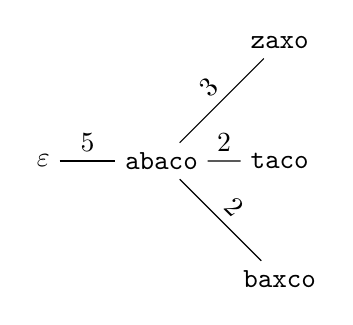
\begin{tikzpicture}[grow=right, sloped]
    \node[draw=none,fill=none] {$\varepsilon$}
        child {
            node[draw=none,fill=none] {\tt abaco}
                child {
                    node[draw=none,fill=none] {\tt baxco}
                    edge from parent
                    node[above] {2}
                }
                child {
                    node[draw=none,fill=none] {\tt taco}
                    edge from parent
                    node[above] {2}
                }
                child {
                    node[draw=none,fill=none] {\tt zaxo}
                    edge from parent
                    node[above] {3}
                }
                edge from parent
                node[above] {5}
        };
    \end{tikzpicture}
  \end{figure}

\end{enumerate}

\exercise

You are given the two files: $f_{old} = \texttt{"cane gatto orso"}$, $f_{new} =
\texttt{"cane matto dorso"}$, and assume a block size $B = 3$ chars.
%
\begin{itemize}

  \item Show the execution of the algorithm rsync
  \emph{(comment the various steps)}.

  \item Show the execution of the algorithm zsync
  \emph{(comment the various steps)}.

\end{itemize}

\solution

\begin{description}

  \item[rsync] Client starts computing the hashes of $f_{old}$ divided by blocks
  of 3 chars:
  %
  \begin{align*}
    \underbracket{\vphantom{\tt g}\texttt{c a n}}_{H_1}\
    \underbracket{\texttt{e \_ g}}_{H_2}\
    \underbracket{\vphantom{\tt g}\texttt{a t t}}_{H_3}\
    \underbracket{\vphantom{\tt g}\texttt{o \_ o}}_{H_4}\
    \underbracket{\vphantom{\tt g}\texttt{r s o}}_{H_5}
  \end{align*}
  %
  The client sends the hashcodes to the server, which compares them to the ones
  produced by the rolling hash on $f_{new}$:
  %
  \begin{align*}
    \underbracket{\vphantom{\tt g}\texttt{c a n}}_{H_1}\ \texttt{e \_ m}\
    \underbracket{\vphantom{\tt g}\texttt{a t t}}_{H_3}\ \texttt{o \_ d o}\
    \underbracket{\vphantom{\tt g}\texttt{r s o}}_{H_5}
  \end{align*}
  %
  The server then sends: $H_1$, "\texttt{e g}", $H_3$, "\texttt{o do}", $H_5$.

  \item[zsync] Server starts computing the hashes of $f_{new}$ divided block by
  block:
  %
  \begin{align*}
    \underbracket{\vphantom{\tt g}\texttt{c a n}}_{H_1}\
    \underbracket{\vphantom{\tt g}\texttt{e \_ m}}_{H_2}\
    \underbracket{\vphantom{\tt g}\texttt{a t t}}_{H_3}\
    \underbracket{\vphantom{\tt g}\texttt{o \_ d}}_{H_4}\
    \underbracket{\vphantom{\tt g}\texttt{o r s}}_{H_5}\
    \underbracket{\vphantom{\tt g}\texttt{o \$}}_{H_6}\
  \end{align*}
  %
  The server sends the hashcodes to the client, which compares them to the ones
  produced by the rolling hash on $f_{old}$:
  %
  \begin{align*}
    \underbracket{\vphantom{\tt g}\texttt{c a n}}_{H_1}\
    \texttt{e \_ g}\
    \underbracket{\vphantom{\tt g}\texttt{a t t}}_{H_3}\
    \texttt{o \_}\
    \underbracket{\vphantom{\tt g}\texttt{o r s}}_{H_5}\
    \underbracket{\vphantom{\tt g}\texttt{o \$}}_{H_6}\
  \end{align*}
  %
  Then client sends the vector: 101011. The server then computes the \emph{gzip}
  of the unmatched substrings given the matched ones:
  %
  \begin{table}[H]
    \centering
    \begin{tabular}{r|lcl}
    \tt{c a n a t t o r s o \$} & \colorbox{yellow}{\tt e}
    {\tt \_ m o \_ d \$} & &
    $\langle 0, 0, \text{\tt e} \rangle$ \\
    \tt{c a n a t t o r s o \$} & {\tt e} \colorbox{yellow}{\tt \_}
    {\tt m o \_ d \$} & & $\langle 0, 0, \text{\tt \_} \rangle$ \\
    \tt{c a n a t t o r s o \$} & {\tt e \_} \colorbox{yellow}{\tt m}
    {\tt o \_ d \$} & & $\langle 0, 0, \text{\tt m} \rangle$ \\
    \tt{c a n a t t o r s} \colorbox{pink}{o}{\tt \$}& {\tt e \_ m}
    \colorbox{yellow}{\tt o \_} {\tt d \$} & &
    $\langle 5, 1, \text{\tt \_} \rangle$ \\
    \tt{c a n a t t o r s o \$} & {\tt e \_ m o \_} \colorbox{yellow}{\tt d}
    {\tt \$} & & $\langle 0, 0, \text{\tt d} \rangle$ \\
    \tt{c a n a t t o r s o \$} & {\tt e \_ m o \_ d} \colorbox{yellow}{\tt \$}
    & & $\langle 0, 0, \text{\tt \$} \rangle$ \\
    \end{tabular}
  \end{table}

\end{description}

\exercise

Compress using zdelta the string $s = "\text{\tt abitacolo}"$ given $t =
"\text{\tt abaco}"$.

\solution

The compression produces the following tuples:
%
\begin{table}[H]
  \centering
  \begin{tabular}{r|lcl}
  \colorbox{pink}{\tt a b} {\tt  a c o} & \colorbox{yellow}{\tt a b i} {\tt t a
  c o l o \$} & & $\langle 5, 2, \text{\tt i} \rangle$ \\
  {\tt a b a c o} & {\tt a b i} \colorbox{yellow}{\tt t} {\tt a
  c o l o \$} & & $\langle 0, 0, \text{\tt t} \rangle$ \\
  {\tt a b}\colorbox{pink}{\tt a c o} & {\tt a b i t} \colorbox{yellow}{\tt a
  c o l} {\tt o \$} & & $\langle 7, 3, \text{\tt l} \rangle$ \\
  {\tt a b a c o} & {\tt a b i t a c} \colorbox{pink}{\tt o} {\tt l}
  \colorbox{yellow}{\tt o \$} & & $\langle 2, 1, \text{\tt \$} \rangle$ \\
  \end{tabular}
\end{table}

\exercise

Show how to synchronize via rsync the new file $f_{old} = \text{\tt
“abacccdac”}$ (on the server) using the old file $f_{new} = \text{\tt
“cabaddaccc”}$ (on the client) and blocks of size 3 chars. Then show the
execution of the algorithm zsync, using blocks of size 2 chars.

\solution

\begin{description}

  \item[rsync] Client starts computing the hashes of $f_{old}$ divided by blocks
  of 3 chars:
  %
  \begin{table}[h]
    \centering
    \begin{tabular}{|c|c|c|}
      \tt{a b a} & \tt{c c c} & \tt{d a c} \\
      $H_1$ & $H_2$ & $H_3$ \\
    \end{tabular}
  \end{table}
  %
  The client sends the hashcodes to the server, which compares them to the ones
  produced by the rolling hash on $f_{new}$:
  %
  \begin{table}[H]
    \centering
    \begin{tabular}{|c|c|c|c|c|}
      \tt{c} & \tt{a b a} & \tt{d} & \tt{d a c} & \tt{c c} \\
      ? & $H_1$ & ? & $H_3$ & ? \\
    \end{tabular}
  \end{table}
  %
  The server then sends: "{\tt c}", $H_1$, "{\tt d}", $H_3$, "{\tt cc}".

  \item[zsync] Server starts computing the hashes of $f_{new}$ divided block by
  block:
  %
  \begin{table}[H]
    \centering
    \begin{tabular}{|c|c|c|c|c|}
      \tt{c a} & \tt{b a} & \tt{d d} & \tt{a c} & \tt{c c} \\
      $H_1$ & $H_2$ & $H_3$ & $H_4$ & $H_5$ \\
    \end{tabular}
  \end{table}
  %
  The server sends the hashcodes to the client, which compares them to the ones
  produced by the rolling hash on $f_{old}$:
  %
  \begin{table}[H]
    \centering
    \begin{tabular}{|c|c|c|c|c|}
      \tt{a} & \tt{b a} & \tt{c c} & \tt{c d} & \tt{a c} \\
      ? & $H_2$ & $H_5$ & ? & $H_4$\\
    \end{tabular}
  \end{table}
  %
  Then client sends the vector: 01011. The server then computes the \emph{gzip}
  of the unmatched substrings given the matched ones:
  %
  \begin{table}[H]
    \centering
    \begin{tabular}{r|lcl}
    \tt{b a a c c}\colorbox{pink}{\tt c} & \colorbox{yellow}{\tt c a } {\tt d d \$} & &
    $\langle 1, 1, \text{\tt a} \rangle$ \\
    \tt{b a a c c c} & {\tt c a } \colorbox{yellow}{\tt d} {\tt d \$} & &
    $\langle 0, 0, \text{\tt d} \rangle$ \\
    \tt{b a a c c c} & {\tt c a } \colorbox{pink}{\tt d} \colorbox{yellow}{\tt d \$} & &
    $\langle 1, 1, \text{\tt \$} \rangle$ \\
    \end{tabular}
  \end{table}

\end{description}

\section{Dictionary Search}
\exercise

Given the dictionary $D = \{\texttt{bingo}, \texttt{bins}, \texttt{box},
\texttt{bull}, \texttt{cat}\}$
%
\begin{itemize}

  \item construct a 3-gram index for $D$ (by guaranteeing $L$ 3-grams per
  $L$-long strings);

  \item describe the algorithm that searches for the strings in $D$ which are at
  1-edit distance from $P = \texttt{binno}$.

\end{itemize}

\solution

We construct the 3-gram index for $D$:
%
% \begin{table}[H]
%   \centering
  \begin{longtable}{ccl}
    \texttt{\$\$b} & $\rightarrow$ & \texttt{bingo}, \texttt{bins},
    \texttt{box}, \texttt{bull} \\
    \texttt{\$\$c} & $\rightarrow$ & \texttt{cat} \\
    \texttt{\$bi} & $\rightarrow$ & \texttt{bingo}, \texttt{bins} \\
    \texttt{\$bo} & $\rightarrow$ & \texttt{box} \\
    \texttt{\$bu} & $\rightarrow$ & \texttt{bull} \\
    \texttt{\$ca} & $\rightarrow$ & \texttt{cat} \\
    \texttt{bin} & $\rightarrow$ & \texttt{bingo}, \texttt{bins} \\
    \texttt{box} & $\rightarrow$ & \texttt{box} \\
    \texttt{bul} & $\rightarrow$ & \texttt{bull} \\
    \texttt{cat} & $\rightarrow$ & \texttt{cat} \\
    \texttt{ing} & $\rightarrow$ & \texttt{bingo} \\
    \texttt{ins} & $\rightarrow$ & \texttt{bins} \\
    \texttt{ngo} & $\rightarrow$ & \texttt{bingo} \\
    \texttt{ull} & $\rightarrow$ & \texttt{bull} \\
    \texttt{BIS\$} & $\rightarrow$ & \texttt{BIS} \\
    \texttt{IS\$B} & $\rightarrow$ & \texttt{BIS} \\
    \texttt{OS\$P} & $\rightarrow$ & \texttt{POS} \\
    \texttt{POS\$} & $\rightarrow$ & \texttt{POS} \\
    \texttt{S\$BI} & $\rightarrow$ & \texttt{BIS} \\
    \texttt{S\$PO} & $\rightarrow$ & \texttt{POS} \\
  \end{longtable}
% \end{table}
%
Then we contruct the 3-grams of the query $P = \texttt{binno}$ and we use them
as a key for the search in the previous index:
%
\begin{table}[H]
  \centering
  \begin{tabular}{ccl}
    \texttt{\$\$b} & $\rightarrow$ & \texttt{bingo}, \texttt{bins},
    \texttt{box}, \texttt{bull} \\
    \texttt{\$bi} & $\rightarrow$ & \texttt{bingo}, \texttt{bins} \\
    \texttt{bin} & $\rightarrow$ & \texttt{bingo}, \texttt{bins} \\
    \texttt{inn} & $\rightarrow$ & $\emptyset$ \\
    \texttt{nno} & $\rightarrow$ & $\emptyset$ \\
  \end{tabular}
\end{table}
%
Since the requested edit distance is $E = 1$, we know that the minimum number of
occurrence of a word in our query must be $|P| - E \cdot k = 5 - 1 \cdot 3 = 2$
to be accepted. We can see that the words \texttt{bingo} and \texttt{bins}
satisfy this condition, while all the other words will be filtered. Since the
results may be a false positive, we check the real edit distance via dynamic
programming, which will produce the following results:
%
\begin{table}[H]
  \centering
  \begin{tabular}{c|c|c|c|c|c|c|}
            &   & {\tt b} & {\tt i} & {\tt n} & {\tt n} & {\tt o} \\ \hline
            & 0 &    1    &    2    &    3    &    4    &    5 \\ \hline
    {\tt b} & 1 &    0    &    1    &    2    &    3    &    4 \\ \hline
    {\tt i} & 2 &    1    &    0    &    1    &    2    &    3 \\ \hline
    {\tt n} & 3 &    2    &    1    &    0    &    1    &    2 \\ \hline
    {\tt g} & 4 &    3    &    2    &    1    &    1    &    1 \\ \hline
    {\tt o} & 5 &    4    &    3    &    2    &    2    & \colorbox{lime}{1} \\
    \hline
  \end{tabular}
  \quad\quad
  \begin{tabular}{c|c|c|c|c|c|c|}
            &   & {\tt b} & {\tt i} & {\tt n} & {\tt n} & {\tt o} \\ \hline
            & 0 &    1    &    2    &    3    &    4    &    5 \\ \hline
    {\tt b} & 1 &    0    &    1    &    2    &    3    &    4 \\ \hline
    {\tt i} & 2 &    1    &    0    &    1    &    2    &    3 \\ \hline
    {\tt n} & 3 &    2    &    1    &    0    &    1    &    2 \\ \hline
    {\tt s} & 4 &    3    &    2    &    1    &    1    & \colorbox{pink}{2} \\
    \hline
  \end{tabular}
\end{table}
%
So, the word \texttt{bingo} is accepted, since it has edit distance 1, while
\texttt{bins} is rejected, since it has edit distance 2.

\exercise

Compute the Permuterm index for the two strings \{\texttt{BIS}, \texttt{POS}\}
and show how it is possible to search for \texttt{P*S} into it.

\solution

First we compute the permuterm index:
%
\begin{longtable}{ccc}
  \texttt{\$BIS} & $\rightarrow$ & \texttt{BIS} \\
  \texttt{\$POS} & $\rightarrow$ & \texttt{POS} \\
  \texttt{BIS\$} & $\rightarrow$ & \texttt{BIS} \\
  \texttt{IS\$B} & $\rightarrow$ & \texttt{BIS} \\
  \texttt{OS\$P} & $\rightarrow$ & \texttt{POS} \\
  \texttt{POS\$} & $\rightarrow$ & \texttt{POS} \\
  \texttt{S\$BI} & $\rightarrow$ & \texttt{BIS} \\
  \texttt{S\$PO} & $\rightarrow$ & \texttt{POS} \\
\end{longtable}
%
Then we transform the query in \texttt{S\$P*}, which will produce the following
result:
%
\begin{table}[H]
  \centering
  \begin{tabular}{ccc}
    \texttt{S\$PO} & $\rightarrow$ & \texttt{POS} \\
  \end{tabular}
\end{table}



\end{document}
